\documentclass[UTF8]{ctexart}
\usepackage{graphicx}
\usepackage{amsmath}
\usepackage{bibentry,natbib}
\usepackage{fancyhdr}

\title{Machine Learning Note}
\author{BrightHush}
\date{\today}

\begin{document}
\maketitle
\tableofcontents

\pagestyle{fancy}
\cfoot{\thepage}

\newcommand{\figref}[1]{\figurename~\ref{#1}}

\section{Logistic Regression}
If given x, we try to predict y($y \in [0, 1]$). We will choose
\[ h_{\theta}(x) = g(\theta ^ T x) = \frac{1}{1+e^{-\theta ^ T x}} \]
where
\[ g(z) = \frac{1}{1 + e^{-z}} \]
is called the \textbf{logistic function} or the \textbf{sigmoid function}.
\par
There is a useful property of the derivative of the sigmoid function.
\[ g^{'}(z) = g(z)(1-g(z)) \]

\par
As before, we are keeping the convention of letting $x_0 = 1$, so 
$\theta ^ T x = x_0 + \sum_{j=1}^n \theta_j x_j$

If we regard $h_{\theta}(x)$ to be the probability of $y$ to be labeled with
1. Then we get 
\[ P(y=1|x;\theta) = h_{\theta}(x) \]
\[ P(y=0|x;\theta) = 1 - h_{\theta}(x) \]
Then we combine these two equations as below
\[ p(y|x;\theta) = (h_{\theta}(x))^y (1-h_{\theta}(x))^{1-y} \]

\par
For the training examples, we can represent the likely hood as 
\begin{align}
L(\theta) &= \Pi_{i=1}^m p(y^{(i)}|x^{(i)};\theta)
\\
&= \pi_{i=1}^m (h_{\theta}(x^i))^{y^i} (1-h_{\theta}(x^i))^{1-y^i}
\end{align}

\par
As before we try to maximize the log likely hood
\begin{align}
\ell(\theta) &= log L(\theta)
\\
&= \sum_{i=1}^m (y^ilog h_{\theta}(x^i) + (1-y^i)log(1-h_{\theta}(x^i)))
\end{align}

\par
To maximize the log likely hood, we use gradient ascent algorithm. Written
in vectorial notation, our updates will therefore be given by 
$\theta := \theta + \alpha \nabla_{\theta}\ell(\theta)$. When working with just
one example $(x, y)$, and take derivatives to derive the stochastic gradient ascent
rule:
\begin{align}
\ell(\theta) &= ylog(h_{\theta}(x)) + (1-y)log(1-h_{\theta}(x))
\\
&= ylog(g_{\theta}(\theta^T x)) + (1-y)log(1-g_{\theta}(\theta^T x))
\end{align}

Then the derivative can be calculated as below
\begin{align}
\frac{\partial}{\partial \theta_j} \ell(\theta) &= 
(\frac{y}{g(\theta^T x)} - \frac{1-y}{1-g(\theta^Tx)})g^{'}(\theta^T x)
\\
&= (y-g(\theta^Tx))x_j
\\
&= (y-h_{\theta}(x))x_j
\end{align}
\par
Thus we get the stochastic gradient ascent rule for example $i$
\[ \theta_j := \theta_j + \alpha(y^i-h_{\theta}(x^i))x_{j}^i \]

\section{Softmax Regression}
相比较于Logistic Regression进行二分类问题,Softmax Regression进行的是多分类问题,也就是y可以去k个不同的
值。因此对于训练集
\[\{(x^{(1)}, y^{(1)}), \cdots, (x^{(m)}, y^{(m)}) \} \ (y^{(i)} \in {1, 2, \cdots, k})\]。
\par
对于每个输入x,我们想估计其为类别j的概率$p(y=j|x, \theta)$,那么我们用一个k维向量表示其对应为每个类别的概率

\begin{equation}
h_{\theta}(x) = 
\left[ 
\begin{array}{c}
p(y=1|x;\theta) \\
p(y=2|x;\theta) \\
\vdots \\
p(y=k|x;\theta)
\end{array}
\right] 
=
\frac{1}{\sum_{j=1}^k e^{\theta_j^T x}}
\left[
\begin{array}{c}
e^{\theta_1^T x} \\
e^{\theta_2^T x} \\
\vdots \\
e^{\theta_k^T x} \\
\end{array}
\right]
\end{equation}
\par
因此
\[ p(y=j|x;\theta) = \frac{e^{\theta_j^T x}}{\sum_{j=1}^k e^{\theta_j^T x}} \]。
参照Logistic Regression合并概率表示方式,我们可以得到Cost Function
\begin{align}
J(\theta) &= -\frac{1}{m} \sum_{i=1}^m \sum_{j=1}^k \{y_i=j\} logp(y=j|x;\theta) \\
&= -\frac{1}{m} \sum_{i=1}^m \sum_{j=1}^k \{y_i=j\} log \frac{e^{\theta_j^T x}}{\sum_{j=1}^k e^{\theta_j^T x}}
\end{align}

\par
对于$J(\theta)$的最小化问题,目前没有闭式解法,因此采用迭代的优化算法(例如梯度下降、L-BFGS等),
对$\theta_j$求导可得
\[ \nabla_{\theta_j}J(\theta) = -\frac{1}{m} \sum_{i=1}^m (1\{y^i=j\}-p(y^i=j|x^i;\theta))x_j^i \]
注意$\theta_j$是一个向量,因此$\nabla_{\theta_j}J(\theta)$也是一个向量,因此在梯度下降过程中我们需要
更新$\theta_j$按照如下方式
\[ \theta_j := \theta_j - \alpha \nabla_{\theta_j} J(\theta) \]
其中\[j \in \{1, \cdots, k\}\]

\par
对于不加正则项的$J(\theta)$,Softmax Regression存在一个参数冗余的问题,因此加上权重衰减项,这个项会惩罚过大的参数,
该衰减项也就是L2正则项。通过添加衰减项可以有效解决这个问题,因此$J(\theta)$函数变为
\begin{align}
J(\theta) &= 
-\frac{1}{m} \sum_{i=1}^m \sum_{j=1}^k \{y_i=j\} log \frac{e^{\theta_j^T x}}{\sum_{j=1}^k e^{\theta_j^T x}}
+ \frac{\lambda}{2} \sum_{i=1}^k \sum_{j=1}^n \theta_{i,j}^2
\end{align}
\par
对新的$J(\theta)$的导数如下计算
\[ \nabla_{\theta_j}J(\theta) = -\frac{1}{m} \sum_{i=1}^m (1\{y^i=j\}-p(y^i=j|x^i;\theta))x_j^i + \lambda \theta_j\]

\section{Softmax Regression and Logistic Regression}
利用Softmax Regression的参数冗余的特点,当k=2,那么可以将Softmax Regression的形式转化为
Logistic Regression的形式,因此可以认为Logistic Regression为Softmax Regression的特殊形式。

\section{Convolutional Neural Network}
卷积神经网络是不同于通常全连接神经网络建模方式,其有以下三个特点:
\begin{itemize}
\item[*] 局部区域感知,也就是非全连接
\item[*] 权重共享,可以有效减少需要训练的参数个数
\item[*] 空间或者时间上的采样,对于图像处理来说,能比较好的获得缩放、旋转等不变性的特点
\end{itemize}

\subsection{Architecture of CNN}
A convolutional neural network consists of several layes. These layers can be of three types:
\begin{itemize}
\item[\textbf{• Convolutional:}] The convolutional layer is just an image convolution of the 
previous layer, where the weights specify the convolution filter. In addition, there may be
several feature maps in each convolutional layer, each map takes inputs from all the maps in
the previous layer, using potentially different filters.

\item[\textbf{• Max Pooling:}] After each convolutional layer, there may be a pooling layer
takes small rectangular blocks from the convolutional layer and sub-sample it to produce a 
single output from that block. There are several ways to do this pooling, such as taking the 
average or the maximum, or a learned linear combination of the neurons in the block.

\item[\textbf{• Fully Connected:}] Finally, after several convolutional and max-pooling layers,
a fully connected layer takes all neurons in the previous layer and connects it to every single 
neuron it has.
 
\end{itemize}

\par
The resulting neural network will look like \ref{Fig:LeNet}
\\
\begin{figure}[h!] 
    \centering     
    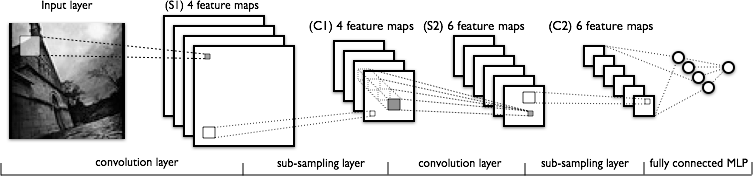
\includegraphics[width=1.2\textwidth]{LeNet}   
    \caption{\label{Fig:LeNet}LeNet Architecture} 
\end{figure}

\subsection{Forward Propagation}
Only differences exist in Convolutional Layer and Max-pooling layer. The forward propagation 
method in fully connected layer is same with usual neural network.

\subsubsection{Convolutional Layers}
Suppose we have some $N \times N$ square neuron layers which is followed by our convolutional 
layer. If we use an $m \times m$ filter $w$, our convolutional layer output will be of size
$(N-m+1) \times (N-m+1)$. We can compute the input to some unit $x_{ij}^l$ in our layer
\[ x_{ij}^l = \sum_{a=0}^{m-1} \sum_{b=0}^{m-1} w_{ab}y_{(i+a)(j+b)}^{l-1} \]
\par
Then apply the non-linearity function
\[ y_{ij}^l = \sigma(x_{ij}^l) \]

\subsubsection{Max-Pooling Layer}
The max-pooling layers are quite simple. They simply take some $k \times k$ region and 
output a single value, for example the maximum value in that region.

\subsection{Backward Propagation}
Backward propagation in fully connected layers are same with neurons in usual neural networks.
So we only concentrate on Convolutional Layer and Max-pooling Layers.

\subsubsection{Convolutional Layers}
Let's assume that we have some error function $E$. Let figure out what the gradient component
is for each weight by applying the chain rule. In the chain rule, we must sum the contributions
of all expressions in which the variable occur
\begin{align}
\frac{\partial E}{\partial w_{ab}} 
&= \sum_{i=0}^{N-m} \sum_{j=0}^{N-m} \frac{\partial E}{\partial x_{ij}^l} \frac{\partial x_{ij}^l}{\partial w_{ab}}
\\
&= \sum_{i=0}^{N-m} \sum_{j=0}^{N-m} \frac{\partial E}{\partial x_{ij}^l} y_{(i+a)(j+b)}^{l-1}
\end{align}

\par
Once more using the chain rule, we can calculate $\frac{\partial E}{\partial x_{ij}^l}$
\begin{align}
\frac{\partial E}{\partial x_{ij}^l} 
&= \frac{\partial E}{\partial y_{ij}^l} \frac{\partial y_{ij}^l}{\partial x_{ij}^l}
\\
&= \frac{\partial E}{\partial y_{ij}^l} \frac{\partial}{\partial x_{ij}^l} (\sigma(x_{ij}^l))
\\
&= \frac{\partial E}{\partial y_{ij}^l} \sigma^{'}(x_{ij}^l)
\end{align}

\par
We need to propagate errors back to the previous layer, we can once use
chain rule to calculate $\frac{\partial E}{\partial y_{ij}^{l-1}}$.
\begin{align}
\frac{\partial E}{\partial y_{ij}^{l-1}} 
&= \sum_{a=0}^{m-1} \sum_{b=0}^{m-1} \frac{\partial E}{\partial x_{i-a,j-b}^l} 
   \frac{\partial x_{i-a,j-b}^l}{\partial y_{ij}^{l-1}}
\\
&= \sum_{a=0}^{m-1} \sum_{b=0}^{m-1} \frac{\partial E}{\partial x_{i-a,j-b}^l} w_{ab}
\end{align}
This looks slightly like convolution.

\subsubsection{Max-Pooling Layers}
We know that $k \times k$ blocks are reduced to a single value in forward propagation.
Then this single value acquires an error computed from backwards propagation from the 
previous layer. This error then just backward to the place where it came from.

\subsection{Conclusion}
Convolutional neural networks are architecturally different way of processing dimensioned
and ordered data. Instead of assuming that the location of the data is irrelevant, covolutional
and max-pooling layer enforce weight sharing. This models the way the human visual cortex works,
and has been shown to work incredibly well for object recognition and a number of other tasks. 

\section{References}
\begin{itemize}
\item[1] Convolutional Neural Networks, \\
\url{http://andrew.gibiansky.com/blog/machine-learning/convolutional-neural-networks/} .
\item[2] 数据挖掘系列(10)卷积神经网络算法的一个实现, \\
\url{http://www.cnblogs.com/fengfenggirl/p/cnn\_ implement.html}.
\item[3] 受限波兹曼机(RBM)学习笔记, \\
\url{http://blog.csdn.net/itplus/article/details/19168937}
\end{itemize}

\end{document}
